\Section{Typography and direction of reading}{}
\lettrine{A}{tlan's} writing system is a natural application of our philosophy: start with elementary parts, and every complexity will be a mere combination of those parts. Our glyphs (as we shall call them) each denote one syllable. They always do so; they always will stand for the {\it same} syllable. Unlike English: in the words \lq\lq tone\rq\rq and  \lq\lq to\rq\rq, the \lq\lq to\rq\rq is pronounced respectively [t\textturnm] and [t\textbaro]. 

That is the rationale behind our writing system; let us dive into the details. As told, Atlan has a set of basic lines. They are:

\begin{center}

\begin{tabular}{c|c| m{1cm} |c}
\hline
\multicolumn{2}{c}{Consonants} & \multicolumn{2}{c}{Vowels} \\ 
\hline
{\bf Line} & {\bf In I.P.A.} & {\bf Line} & {\bf In I.P.A.} \\
\DeclareStroke{\CenterVertical} & ... & \Atlanu & ... \\  
\hline
\DeclareStroke{\CenterHorizontal} & ... &  \Atlani & ... \\ 
\DeclareStroke{\BigNW} & ... & \Atlana & ... \\ 
\DeclareStroke{\BigSW} & ... & \Atlano & ... \\ 
\DeclareStroke{\BigSE} & ... & \Atlane & ... \\
\DeclareStroke{\BigNW} & ... & & \\
\DeclareStroke{\Dot{Center}} & ...& &\\
\DeclareStroke{\MediumCircle{Center}} & ... & & \\
\end{tabular}

\end{center}

These lines all represent a single vowel ({\it V}), or a single consonant ({\it C}). We can combine them to make syllables. By combining two consonant lines, you get a CVC-syllable, such as {\it loj}, {\it pas} or {\it mup}. You can also make a VC-syllable, such as {\it mu}, {\it po}, or {\it ji}. The vowels don't have separate lines in a CVC or VC-syllable; instead, the vowel is determined by the position of the two consonant-lines. We will go deeper into that below. First, we give the rules for the order of the consonants and vowels: what determines whether two lines make e.g. {\it poj} or {\it jop}, {\it mu} or {\it um}? 

This order is determined by the manner in which the lines combine. There is always a \lq\lq bigger \rq\rq line, and a smaller one. These lines fit inside an imaginary box. The position of the smaller line relative to the bigger line, determines the order of consonants. A general rule of thumb is best given with the help of a box:

\begin{center}

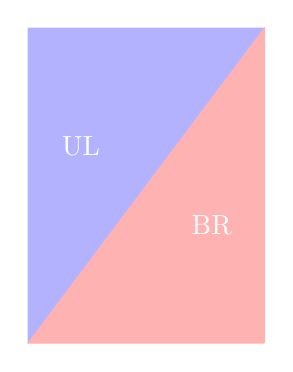
\begin{tikzpicture}
\draw[blue!30, fill= blue!30] (0,0) -- (3,4) -- (0,4) -- (0,0);
\draw[red!30,fill =red!30] (3,0) -- (3,4) -- (0,0) -- (3,0);
\node(A) at (0.67,2.5){\color{white} UL};
\node(B) at (2.33,1.5){\color{white} BR};
\end{tikzpicture}

{\it \footnotesize Figure 1: Box for determining consonant order.}
\end{center}

If the smaller line is in the upper-left triangle (UL), it the consonant it designates comes first. If it is in the bottom-right one, it comes second. For the rest of the explanation, it is advised to keep this box in the back of your head. An example:

\def\restorecorps{\renewcommand{\corpsgrootte}{20pt}}
\begin{wrapfigure}[7]{l}{0.4\textwidth}
\renewcommand{\corpsgrootte}{100pt}
\kus
\restorecorps
\end{wrapfigure}

As you see here, the smaller line is found on top. Hence, it is placed inside the upper-left triangle. The consonant for which the smaller horizontal line stands (the {\it k}), comes before the other consonant, the {\it s}.

\phantom{}

\begin{center}
\definecolor{melon}{RGB}{255,179,179}
\definecolor{caian}{RGB}{204,255,247}
\definecolor{lavender}{RGB}{242,179,255}
\definecolor{jasmine}{RGB}{255,212,128}
\definecolor{lemon}{RGB}{255,247,204}
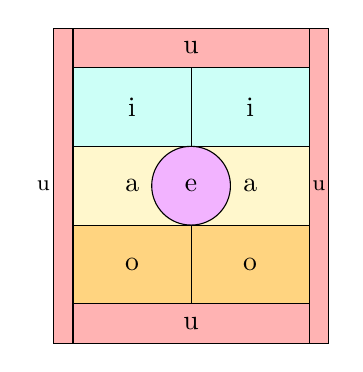
\begin{tikzpicture}
\draw[black] (0,0) rectangle (3,4);
\draw[fill = melon] (0,4) rectangle (3,3.5);
\draw[fill = melon] (0,0.5) rectangle (3,0);
\draw[fill = melon] (-0.25, 0) rectangle (0,4);
\draw[fill = melon] (3.25, 0) rectangle (3,4);
\draw[fill = caian] (1.5,2.5) rectangle (0,3.5);
\draw[fill = caian] (1.5,2.5) rectangle (3,3.5);
\draw[fill = jasmine] (1.5,1.5) rectangle (0,0.5);
\draw[fill = jasmine] (1.5,1.5) rectangle (3,0.5);
\draw[fill = lemon] (1.5,1.5) rectangle (0,2.5);
\draw[fill = lemon] (1.5,1.5) rectangle (3,2.5);
\draw[fill = lavender] (1.5,2) circle (0.5);
\node at (1.5,3.75){u};
\node at (0.75,3){i};
\node at (2.25,3){i};
\node at (0.75,2){a};
\node at (2.25,2){a};
\node at (0.75,1){o};
\node at (2.25,1){o};
\node at (1.5,0.25){u};
\node at (1.5,2){e};
\node at (-0.375, 2){\footnotesize u};
\node at (3.125, 2){\footnotesize u};
\end{tikzpicture}
\end{center}

The vowel is...
\begin{itemize}
\item {\it u} if the smaller line is found at the edges. The smaller line is in its whole above, under, left or right of the main line. 

\item {\it i} if the smaller line is found on the upper-left or upper-right side of the main line. It is usually smaller than the line made for {\it u}, to avoid confusion. 

\item {\it a} if the smaller line is found left or right to the middle of the line. 

\item {\it o} if the smaller line is found on the bottom-left or bottom-right hand of the main line. Again, this line is smaller than the line for {\it u}. 

\item{\it e} if the smaller line is placed in the middle. Or, if the small line intersects with the main line at the middle. In some instances, the small line is then split up by the main line.  
\end{itemize}

Then we have a single exception. You can combine two equivalent lines, to make syllables such as {\it pop}, {\it mum}, or {\it lol}. The order of these lines doesn't matter; hence we choose place the smaller line to the upper-left of the main line in such cases. For the vowel {\it u}, there are two small lines, split at the center. For {\it e}, there are either two or three small lines. At least one of those lines crosses through the center of the imaginary box.
%EXAMPLE>?

Remember that the {\it p} is represented by the dot \DeclareStroke{\Dot{Center}} . For clarity, we couldn't combine simply two dots to make a full syllable. Hence, 


These are the rules. 

\Section{Numerals and Mathmatics}{}


\Section{Font in \TeX}{Jarno Smets}


\Section{On Dyslexia}{Stijn Janssens and Jonathan Roose}

\Section{Cartouche}{}


